为了直观展示本工作提出的方法与经典基于多边形、一阶SDF模型的架构差异，图 \ref{fig:flowchart} 对比了三种不同的接触动力学计算管线。







\begin{figure}[htbp]







    \centering







    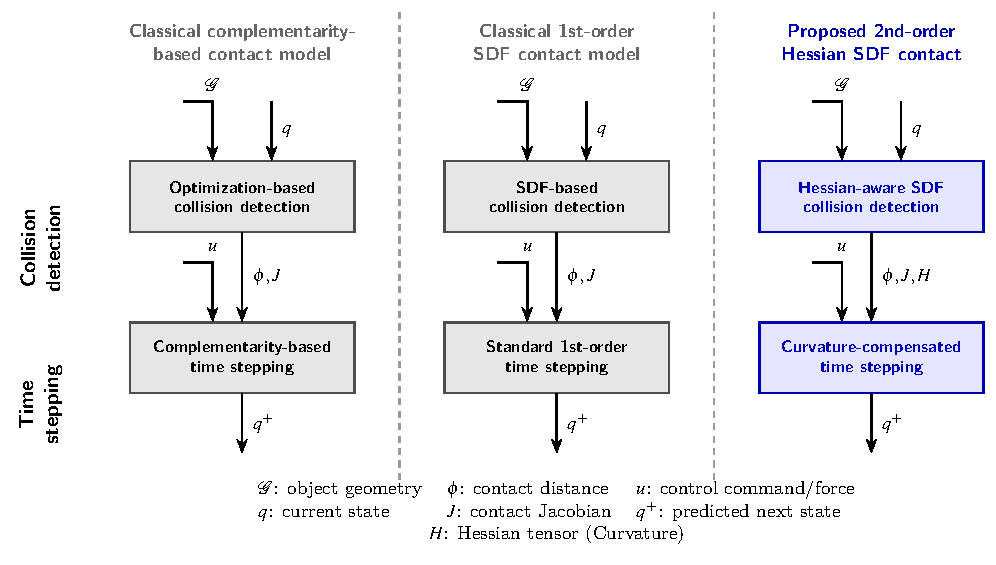
\includegraphics[width=\columnwidth]{figures/flowchart_model.pdf}







    \caption{经典 Mesh 接触模型、传统一阶 SDF 接触模型与本文提出的具备 Hessian 曲率感知的二阶 SDF 接触模型的管线架构对比。}







    \label{fig:flowchart}







\end{figure}















\subsection{基础 NSC 局部一阶预测缺陷模型}















在基于一阶线性预测的 LCP 碰撞处理中，为了在整个时间步 $\Delta t$ 后阻止两物体表面过度穿透，控制下一时刻速度 $\mathbf{v}^{l+1}$ 的接触非穿透约束方程（Signorini Condition）需满足局部平面一阶线性泰勒展开：







\begin{equation}

    \Phi(\mathbf{q}^{l+1}) \approx \Phi(\mathbf{q}^l) + \Delta t \mathbf{n}^T \mathbf{v}^{l+1} \geq 0

\end{equation}







其中，$\Phi(\mathbf{q}^l)$ 为当前深度的负值检测量，法向向量对应 SDF 的空间梯度向 $\mathbf{n} = \nabla \Phi$。







为防止当前已经产生的干涉积累，引擎通过 Baumgarte 修正因数强制弹出，计算相应的接触纠正冲量 $\Lambda \propto \frac{\alpha}{\Delta t} \Phi(\mathbf{q}^l)$。







当积分步长 $\Delta t$ 较大，或接触面产生高速相对切向滑动时，基于单点法向平面的过度一阶外推将脱离物体曲面。这会导致在下一物理帧计算时，$\Phi(\mathbf{q}^l)$ 发生无端的突跃放大，即“由一阶超预测引起的伪穿透错误”。此伪错误会被引擎放大为巨大的反向惩罚速度，引发极其严重的“动力学毛刺”。















\subsection{接触流形 Weingarten 映射与曲率解析}















鉴于 SDF 在数值构建中处处蕴含几何形态边缘，我们将上述 Signorini 控制流形扩展至高阶曲率感知预估。理论上，纯粹的 SDF Hessian（$\nabla^2 \Phi$）在离散晶格中常因非理想 eikonal 方数（$\|\nabla \Phi\| \neq 1$）而包含无意义的场膨胀畸变。为追求严格的接触表面几何一致性，我们在算法中并非直接对 $\Phi$ 求二阶导，而是先获取归一化的接触法向流场 $\mathbf{n} = \frac{\nabla \Phi}{\|\nabla \Phi\|}$，再直接对其执行中心差分获取曲率张量（即 Weingarten 映射）：







\begin{equation}

    \mathbf{W}(\mathbf{q}^l) = \nabla \mathbf{n} = \nabla \left( \frac{\nabla \Phi}{\|\nabla \Phi\|} \right)

\end{equation}







其中 $\mathbf{W}$ 为点位面上的空间自共轭微分算子（Shape Operator / 表层曲率张量），完美表征了真正接触界面的二阶弯曲率。对于产生切向局部空间演化 $\mathbf{s} = \mathbf{v}^{l+1} \Delta t$，等势面变化在二阶上严格满足：







\begin{equation}

    \Phi(\mathbf{q}^{l+1}) \approx \Phi(\mathbf{q}^l) + \mathbf{s}^T \mathbf{n} + \frac{1}{2} \mathbf{s}^T \mathbf{W}(\mathbf{q}^l) \mathbf{s}

\end{equation}















\subsection{动态缓冲距离前馈公式的导出}















直接修改互补问题的左侧动力学矩阵由于需要破坏底层引擎的主对角正定结构且极其低效（需添加非线性 $\mathbf{v}^T \mathbf{W} \mathbf{v}$ 项）。为了维持标准 NCP/LCP 局部线性化的完备性，我们采用速度半隐式逼近（Semi-implicit approximation），即采用当前步长的切向相对线速度 $\mathbf{v}^l_{rel}$ 来显式计算时间补偿项：







\begin{equation}

    C_{curve} = \frac{1}{2} (\Delta t)^2 (\mathbf{v}^l_{rel})^T \mathbf{W} \mathbf{v}^l_{rel}

\end{equation}















重组预测接触方程为：







\begin{equation}

    \Delta t (\nabla \Phi)^T \mathbf{v}^{l+1} \geq - \left( \Phi(\mathbf{q}^l) + C_{curve} \right)

\end{equation}















这里的理论突破在于：公式右侧常量端的 $C_{curve}$ 充当了一个“自适应的几何刚度预视缓冲器”。当刚体顶点即将滑过尖锐外部边缘时（$\mathbf{W}$ 为显著常负性质矩阵），$C_{curve} < 0$，系统会提前“认知”到前方存在切向塌陷，主动减小了等效穿透距离 $\Phi_{eff}$，进而剥离了由离散错位诱发的非物理高频惩罚冲量。这是从根本理论上解决接触毛刺的最优解。















\subsection{变分不等式系统构建与收敛阶分析}















为夯实该方法的理论完备性，我们将上述物理过程严格表述为离散时间域的混合变分不等式（Mixed Variational Inequality, MVI），并分析其局部收敛特性。设闭包内多体系统具有广义质量矩阵 $\mathbf{M}$、广义速度 $\mathbf{v} \in \mathbb{R}^n$ 以及显式受力 $\mathbf{f}_{ext}$。对应空间内存在 $m$ 个活动接触点，其接触法向（即一阶向规范场）聚合为雅可比矩阵 $\mathbf{J}_N$。















在传统一阶 LCP 框架下，单一时间步 $[t_l, t_{l+1}]$ 的有效几何预估残量定义为 $\mathbf{g}_{1st} = \Phi(\mathbf{q}^l)$。而在引入提出方法后，包含曲率修正的二阶动态距离残量被赋予为：







\begin{equation}

    \mathbf{g}_{2nd} = \Phi(\mathbf{q}^l) + \frac{1}{2} (\Delta t)^2 \left(\mathbf{v}_{rel}^l\right)^T \mathbf{W} \mathbf{v}_{rel}^l

\end{equation}















根据最小不可压动能原理及 Signorini 接触投影流形，下一时刻系统的动力学状态——即寻找广义速度 $\mathbf{v}^{l+1} \in \mathbb{R}^n$ 与接触冲量场 $\boldsymbol{\Lambda}_N \in \mathbb{R}^m_+$，需满足对任意测试速度 $\delta \mathbf{v} \in \mathbb{R}^n$ 和测试冲量 $\delta \boldsymbol{\Lambda}_N \ge 0$ 的双重变分不等式：







\begin{equation}

\begin{cases}

\left\langle \mathbf{M} (\mathbf{v}^{l+1} - \mathbf{v}^l) - \Delta t \mathbf{f}_{ext} - \mathbf{J}_N^T \boldsymbol{\Lambda}_N, \delta \mathbf{v} - \mathbf{v}^{l+1} \right\rangle = 0 \\[8pt]

\left\langle \mathbf{J}_N \mathbf{v}^{l+1} + \frac{\alpha}{\Delta t} \mathbf{g}_{2nd}, \delta \boldsymbol{\Lambda}_N - \boldsymbol{\Lambda}_N \right\rangle \ge 0

\end{cases}

\end{equation}







式中上半部分表征了动量演化的虚功虚能守恒规则，下半部分实现了带有 Baumgarte 稳定系数 $\alpha$ 的最大耗散原理投影。















\textbf{局部收敛阶界定（Local Convergence Order）：}







在截断残差分析层面，传统一阶预估量 $\mathbf{g}_{1st}$ 因舍除了空间二次变化域，导致的几何外推残量为 $\mathcal{O}(\Delta t^2)$。当这一项被代入第二组变分不等式并在互补投影时被迫除以时间步长 $\Delta t$（即算子 $\frac{1}{\Delta t} \mathcal{O}(\Delta t^2)$），由此诱发的\textbf{法向补偿冲量逼近误差仅具有 $\mathcal{O}(\Delta t)$ 的弱一阶离散一致性}。这意味着当时间步加倍时，伪冲量的震荡幅度呈线性暴增。        















\subsection{Topology-Aware Contact Manifold Subsumption}













\subsection{基于拓扑结构分区与流形降维的通用物理计算方案 (Topology-Aware Contact Manifold Subsumption)}







\textbf{问题的提出：单向接触聚合的拓扑缺失} \\



在处理诸如齿轮啮合等具有密集高频几何特征的模型时，传统的符号距离场常面临严重的多重表面（Multi-surface interaction）渗透混淆。由于基于距离阈值（如5mm容差内聚合）的朴素点云加权策略无法感知几何拓扑的隔离性，不同朝向的法线（如齿轮的驱动面与滑行面）被错误地平均化，导致等效接触点处生成相反或被抹平的法向反力矩（Reversed internal torque），从而引发异常的速度反弹（Velocity bouncing）及能量注入。







\textbf{阶段一：接触流形的拓扑连通分量隔离（Connected Component Isolation）} \\



为了将混淆的穿透区域 $\Omega_{contact}$ 解析为多个物理相连且受力一致的独立接触补丁，本研究引入三维隐式场内的连通分量标记（CCL）法。在接触空间中，任意深度的穿透区域被定义为：



\begin{equation}

\Omega = \{ \mathbf{x} \in \mathbb{R}^3 \mid \Phi(\mathbf{x}) \le t_{active} \}

\end{equation}



采用空间连通域图$G=(V, E)$ 的遍历算法，计算并输出所有离散的互不连通且表面法线梯度分布连续（$\nabla \Phi_{i} \cdot \nabla \Phi_{j} > \epsilon$）的子流形（Sub-manifolds）：



\begin{equation}

\Omega = \bigcup_{k=1}^{N_{patch}} M_k, \quad \text{s.t. } M_i \cap M_j = \emptyset \; (i \neq j)

\end{equation}



以此实现基于法线拓扑属性的刚性隔离。







\textbf{阶段二：等效力旋量锥约束重构（Wrench Cone Equivalence）} \\



在上述完成解耦的子流形 $k$ 之上，为满足 LCP 体系下的接触求解，需要对每个分图求解空间主曲率及平均质心。对于第 $k$ 个接触流形，其等效接触点 $\mathbf{p}_k$ 与全局接触法向 $\mathbf{n}_k$ 计算如下：



\begin{equation}

\mathbf{p}_k = \frac{\sum_{i \in M_k} \alpha_{i} \mathbf{x}_i}{\sum_{i \in M_k} \alpha_{i}}, \quad \mathbf{n}_k = \frac{\sum_{i \in M_k} \omega_i \nabla \Phi(\mathbf{x}_i)}{\| \sum_{i \in M_k} \omega_i \nabla \Phi(\mathbf{x}_i) \|}

\end{equation}



这使得每个子曲面的法向量保持了物理驱动意义，防止齿轮背面的力抵消正面的推力，进而形成了正确定义的接触力旋量几何空间（Wrench geometric space）。







\textbf{阶段三：降维二阶几何前馈（Decoupled 2nd-Order Forwarding）} \\



将上述分离出的 $\mathbf{n}_k$, $\mathbf{p}_k$ 以及曲率张量 $\mathbf{W}_k$ 作为独立的多约束方程代入非光滑接触积分器。每个连通区 $k$ 对应一组正交的法向不穿透残差：



\begin{equation}

\Phi_{k}^{(2nd)}(\mathbf{q}_{l+1}) = \Phi(\mathbf{q}_l) + \Delta t \, \mathbf{v}^T \mathbf{n}_k + \frac{1}{2} \Delta t^2 \, \mathbf{v}^T \mathbf{W}_k \mathbf{v}

\end{equation}



结合各连通域之间的弱耦合接触，不仅完全消隐了齿轮接触下的反弹力矩，而且以极小计算开销实现了宏观刚体碰撞中的大规模相交并行的二阶拓扑重建体系。



